\documentclass[11pt,xcolor={dvipsnames},hyperref={pdftex,pdfpagemode=UseNone,hidelinks,pdfdisplaydoctitle=true},usepdftitle=false]{beamer}

\usepackage{microtype}
\usepackage[slovak]{babel}
\usepackage[utf8]{inputenc}
\usepackage[T1]{fontenc}

\usepackage{caption}
\usepackage{subcaption}
\usepackage{multicol}
\usepackage[export]{adjustbox}
\usepackage[normalem]{ulem}

\usetheme[
nogauge,
%nologo,
nomail,
%amurmapleblue
]{Amurmaple}


\title[SPAR]{SPAR - Systém na podporu analýzy rizík}
\author[A.~Kica]{Bc. Anton Kica}
\institute[FMFI]{FMFI\\Univerzita Komenského v Bratislave}
\date{12. jún, 2026}
\titlegraphic{
\includegraphics[width=4cm]{images/logo.png}}
\collaboration{školiteľ: doc. RNDr. Daniel Olejár, PhD}

%\bibliography{biblio.bib}
\usefonttheme{serif}

\begin{document}

\maketitle
%\sepframe[title={Obsah}]

\begin{frame}
	\frametitle{Čo to je KIB?}
	\textit{Kybernetická a informačná bezpečnosť} (KIB) je multidisciplinárna oblasť zaoberajúca sa skúmaním hrozieb voči informáciám,
	informačným systémom a sieťam a návrhom riešení, ktoré by naplneniu hrozieb zamedzili alebo aspoň zmiernili ich dopad.
\end{frame}


\begin{frame}
	\frametitle{Prečo sa zaoberáme KIB?}
	\begin{itemize}
		\item potrebujeme ochraňovať aktíva pred (ne)úmyselnými hrozbami
		\item najmä základné hodnoty: dôvernosť, integritu a dostupnosť
		\item riešime z dôvodu:
			\begin{itemize}
				\item vlastná potreba obmedziť neželané negatívne potenciálne dopady hrozieb
				\item povinnosti KIB vyplyvajúce z legislatívy Slovenskej republiky (ZoKB a ZoITVS) a Európskej únie (NIS2)
			\end{itemize}
	\end{itemize}
\end{frame}
\begin{frame}
	\frametitle{Ako môžeme riešiť KIB?}
	\begin{itemize}
		\item technické pomôcky, HW, SW
		\item manažérske/organizačné procesy \textbf{$\leftarrow$ naše zameranie}
	\end{itemize}
	\begin{figure}
		
\includegraphics[height=4cm]{images/ISO-27000-Hero-2.jpg}
	\end{figure}
\end{frame}
\begin{frame}
	\frametitle{Naša motivácia}
	\begin{itemize}
		\item nedostatok odborníkov na pokrytie verejných inštitúcii SR (cca. 20 000)
		\item objektívne hrozby, ktoré boli nedávno naplnené
		\item vieme pomôcť laikovi manažérovi KIB splniť si svoje povinnosti?
		\item v bakalárskej práci: čo to znamená vytvoriť systém na pomoc pri zavádzaní ISMS?
		\item \textbf{v diplomovej práci}: čo to znamená vytvoriť systém na analýzu rizík?
	\end{itemize}
\end{frame}
\begin{frame}
	\frametitle{Ciele}
	\begin{enumerate}
		\item \textcolor{Orange}{vysvetlenie zákonných povinností}
		\item \textcolor{OliveGreen}{popísať postup AR}
		\item \textcolor{OliveGreen}{pomôcť pre aktívum vykonať AR}
		\item \textcolor{OliveGreen}{dokumentácia procesu AR}
	\end{enumerate}
\end{frame}
\begin{frame}
	\frametitle{Cieľ: vysvetlenie zákonných povinností}
	\begin{itemize}
		\item nepodarilo sa nám splniť
		\item veľká dynamika, NIS2
		\item novelizácia ZoKB cez 318/2025 Z. z., november 2025
		\item novelizácia ZoITVS cez 67/2026 Z. z., apríl 2026
	\end{itemize}
\end{frame}


\begin{frame}
	\frametitle{Medzinárodné normy a analýza rizík}
	\begin{itemize}
		\item existuje niekoľko noriem a štandardov zaoberajúce sa KIB
		\item séria ISO/IEC 27000
		\item špeciálne publikácie NIST 800
		\item \textbf{metodika BSI IT-Grundschutz}
	\end{itemize}
\end{frame}
\begin{frame}
	\frametitle{vzťah legislatívy a noriem}
	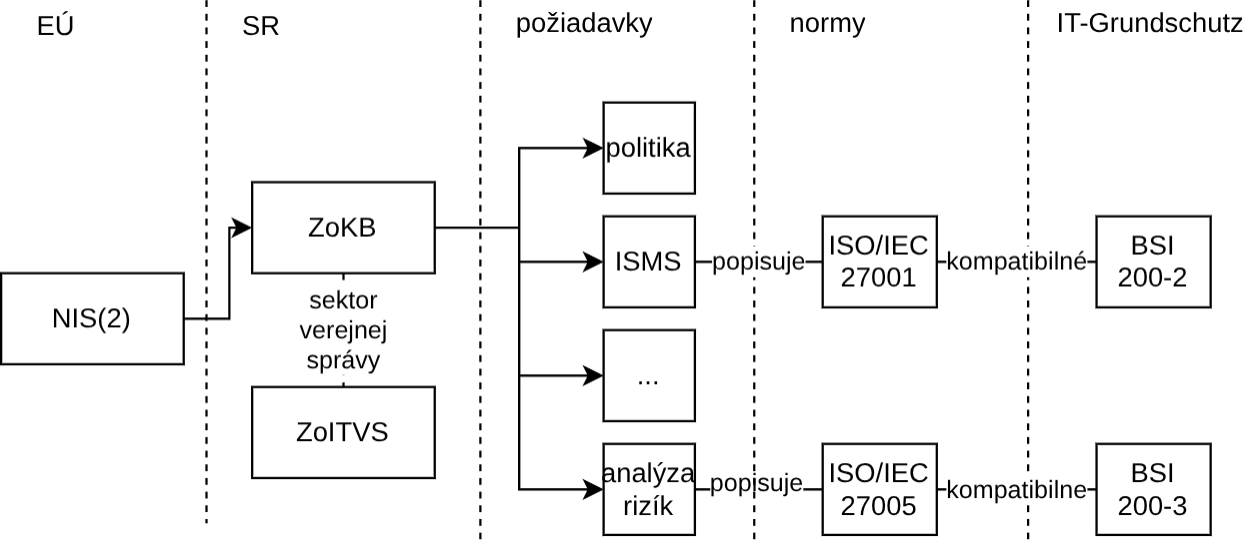
\includegraphics[width=\textwidth]{images/legnorm.png}
\end{frame}

\begin{frame}
	\frametitle{Čo to je analýza rizík?}
	\begin{itemize}
		\item v organizácií/inštutúcií máme aktíva
		\item aktíva majú požiadavky na ochranu základných hodnôť CIA (dôvernosti, integrity a dostupnosti)
		\item hrozby ohrozujú aktíva, potenciálne riziko
		\item riziká potrebujeme ošetriť, znížiť na prijateľnú úroveň
		\item podľa BSI 200-3 proces z krokov:
			\begin{enumerate}
				\item identifikácia hrozieb
				\item klasifikácia rizík
				\item ošetrenie rizík
				\item konsolidácia
			\end{enumerate}
	\end{itemize}
\end{frame}
\begin{frame}
	\frametitle{Analýzy rizík ako súčasť ISMS}
	\begin{multicols}{2}
		\begin{figure}
		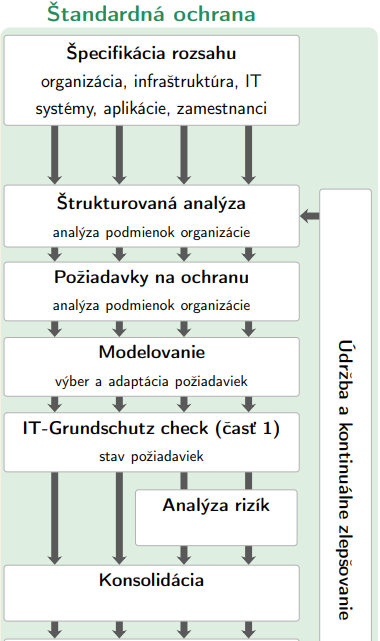
\includegraphics[width=0.35\textwidth]{images/standard-protection.png}
		\caption{Koncept štandardnej ochrany podľa BSI 200-3}
		\end{figure}
		\columnbreak
		\begin{itemize}
			\item systém riadenia informačnej bezpečnosti (ISMS)
			\item systematické riešenie KIB v organizácii
			\item politika, manažér KIB, bezpečnostné roly, opatrenia \ldots
		\end{itemize}
	\end{multicols}
\end{frame}
%\include{00-.tex}

\begin{frame}
	\frametitle{Navrhnutý systém}
	Špecifikácia, nástroje, achitektúra a výsledný \textit{proof-of-concept} \ldots
\end{frame}

\begin{frame}
	\frametitle{Navrhnutý systém: Špecifikácia}
	\begin{itemize}
		\item cielená skupina je menšia organizácia
		\item užívateľ je manažér KIB (m-KIB)
		\item predpokladáme základné znalosti IT a porozumenie informačnej bezpečnosti
		\item systém pomôže m-KIB:
			\begin{itemize}
				\item usmerňovať používateľa v procese analýzy rizík
				\item postupne zbierať informácie získané v procese analýzy rizík
				\item pomôcť koncentrovať údaje v databáze
				\item zjednodušiť manipuláciu s rozsiahlym počtom hrozieb a opatrení
				\item poskytnúť dokumentáciu zavedených bezpečnostných opatrení
			\end{itemize}
	\end{itemize}
\end{frame}
\begin{frame}
	\frametitle{Navrhnutý systém: Špecifikácia}
	\begin{itemize}
		\item predpokladamé vykonanú štrukturovaná analýzu a namodelovanie aktív
		\item \textcolor{BlueViolet}{vstup: zoznam aktív}
			\begin{itemize}
				\item názov
				\item mapovanie na modul
				\item požiadavky na CIA
			\end{itemize}
		\item \textcolor{RedViolet}{výstup: zoznam opatrení}
			\begin{itemize}
				\item typ opatrenia
				\item aplikované na modul? hrozbu?
				\item popis opatrenia
				\item stav implementácie
			\end{itemize}
	\end{itemize}
\end{frame}
\begin{frame}
	\frametitle{Navrhnutý systém: Nástroje a architektúra}
	\begin{itemize}
		\item webová aplikácia, klient a server
		\item HTML5, JavaScript, Booststrap, SvelteKit
		\item Rust, ActixWeb, SQLx
		\item PostgreSQL
	\end{itemize}
\end{frame}
\begin{frame}
	\frametitle{Navrhnutý systém: Ukážka}
	\begin{figure}
		\includegraphics[width=\textwidth]{images/wf/0-asset.png}
	\end{figure}
\end{frame}
\begin{frame}
	\frametitle{Navrhnutý systém: Zoznam analýz}
	\begin{figure}
		\includegraphics[width=\textwidth]{images/wf/spar.png}
	\end{figure}
\end{frame}
\begin{frame}
	\frametitle{Navrhnutý systém: Proces analýzy rizík}
	\begin{figure}
		\includegraphics[width=0.9\textwidth]{images/wf/0-ra.png}
	\end{figure}
\end{frame}
\begin{frame}
	\frametitle{1. Identifikácia hrozieb: katalog hrozieb}
	\begin{figure}
		\includegraphics[width=\textwidth]{images/wf/01-thrid.png}
	\end{figure}
\end{frame}
\begin{frame}
\frametitle{1. Identifikácia hrozieb: špecifická hrozba}
	\begin{figure}
		\includegraphics[height=6cm]{images/wf/02-spfthr.png}
	\end{figure}
\end{frame}
\begin{frame}
\frametitle{1. Identifikácia hrozieb: prehľad}
	\begin{figure}
		\includegraphics[width=\textwidth]{images/wf/03-thrsummary.png}
	\end{figure}
\end{frame}
\begin{frame}
\frametitle{2. Klasifikácia rizík: aktívum a hrozba}
	\begin{figure}
		\includegraphics[height=6cm]{images/wf/11-classification.png}
	\end{figure}
\end{frame}
\begin{frame}
\frametitle{2. Klasifikácia rizík: prehľad}
	\begin{figure}
		\includegraphics[width=0.9\textwidth]{images/wf/12-riskoverview.png}
	\end{figure}
\end{frame}
\begin{frame}
\frametitle{3. Ošetrenie rizík: prehľad}
	\begin{figure}
		\includegraphics[width=\textwidth]{images/wf/24-overview.png}
	\end{figure}
\end{frame}
\begin{frame}
\frametitle{3. Ošetrenie rizík: opatrenia modulu}
	\begin{figure}
		\includegraphics[width=0.9\textwidth]{images/wf/23-modtrm.png}
	\end{figure}
\end{frame}
\begin{frame}
\frametitle{3. Ošetrenie rizík: akceptovanie}
	\begin{figure}
		\includegraphics[width=0.9\textwidth]{images/wf/22-riskaccept.png}
	\end{figure}
\end{frame}
\begin{frame}
\frametitle{4. Kontrola IT-Grundschutz}
	\begin{figure}
		\includegraphics[width=0.9\textwidth]{images/wf/31-check.png}
	\end{figure}
\end{frame}
\begin{frame}
\frametitle{5. Zhrnutie opatrení}
	\begin{figure}
		\includegraphics[width=0.9\textwidth]{images/wf/41-result.png}
	\end{figure}
\end{frame}
\newcommand\pro{\item[\textcolor{PineGreen}{$+$}]}
\begin{frame}[allowframebreaks]
	\frametitle{Porovnanie s BSI 200-3}
	\begin{enumerate}
		\item Identifikácia relevantných hrozieb per aktívum
			\begin{itemize}
				\item elementárne hrozby
				\item špecifické hrozby
			\end{itemize}
		\item Klasifikácia rizík per aktívum a hrozbu
			\begin{itemize}
				\item kvalitatívne; frekvencia a dopad $\rightarrow$ riziko
			\end{itemize}
		\item Ošetrenie rizík per aktívum a hrozbu
			\begin{itemize}
				\item akceptovaním, vyhnutím sa, redukovanim alebo prenesením
			\end{itemize}
		\item Kontrola IT-Grundschutz per opatrenie
			\begin{itemize}
				\item implementované, neimplementované, čiastočne alebo redundantné
			\end{itemize}
		\item Zhrnutie opatrení
	\end{enumerate}
	\pagebreak
	\begin{enumerate}
		 \pro granularita akvívum $\rightarrow$ modul
		 \pro kopírovanie postupu
	\end{enumerate}
	\begin{enumerate}
		\item Identifikácia relevantných hrozieb per \textcolor{PineGreen}{modul}
			\begin{itemize}
				\item elementárne hrozby \textcolor{PineGreen}{explicitne rozdelené na priame a nepriame}
				\item špecifické hrozby
				\pro kategorizácia podľa 27005
			\end{itemize}
		\item Klasifikácia rizík per \textcolor{PineGreen}{modul} a hrozbu
			\begin{itemize}
				\item kvalitatívne; frekvencia a dopad $\rightarrow$ riziko
				\pro tabuľka na relativizáciu rizík
			\end{itemize}
		\pagebreak
		\item Ošetrenie rizík \sout{\textcolor{Red}{aktívum a hrozbu}}
			\begin{itemize}
				\pro modul a hrozba: akceptovaním, vyhnutím sa, redukovanim alebo prenesením
				\pro hrozba: akceptovaním, vyhnutím sa, redukovanim alebo prenesením
				\pro modul: redukovaním z katalógu GSK
				\pro plošne: redukovaním
			\end{itemize}
		\item Kontrola IT-Grundschutz per opatrenie
			\begin{itemize}
				\item implementované, neimplementované, čiastočne alebo redundantné
			\end{itemize}
		\item \textcolor{PineGreen}{Zhrnutie opatrení}
	\end{enumerate}
\end{frame}
\begin{frame}
	\frametitle{Čo sa nám nepodarilo?}
	\begin{itemize}
		\item uspokojivá integrácia výkladu
		\item systém musí m-KIB použiť za sprievodi písomnej časti alebo BSI 200-3
	\end{itemize}
	\begin{figure}
		
\includegraphics[width=0.65\textwidth]{images/learning-mode.png}
		\caption{Vysvetlenie ošetrenia redukovaním prevzaté verbatim z prísomnej časti}
	\end{figure}
\end{frame}
\begin{frame}
	\frametitle{Ďalšie problémy na preskúmanie}
	\begin{itemize}
		\item zapracovanie bezpečnostných incidentov
		\item kvantifikácia človekohodín a finančných nákladov
		\item integrácia do TAXII/STIX, automatizovaná výmena informácií o hrozbách
	\end{itemize}
\end{frame}
\begin{frame}
	\frametitle{Zhrnutie a záver}
	\begin{itemize}
		\item vysvetlili sme analýzu rizík
		\item implementovali sme \textit{proof-of-concept} SPAR
		\item získali sme prehľad na implementáciu plnohodnotného systému
		\item identifikovali sme ďalšie potenciálne problémy na preskúmanie
	\end{itemize}
\end{frame}

\begin{frame}
	\frametitle{ďakujem za pozornosť}
\end{frame}
\begin{frame}
	\frametitle{Odpoveďe na otázky oponenta}
\end{frame}
\begin{frame}
	\frametitle{Diskusia}
	Sú nejaké otázky?
\end{frame}
\end{document}
